\documentclass{ximera}

\input{../../preamble.tex}

\author{Elizabeth Campolongo}

\begin{document}
\begin{exercise}

You have been marooned on an island and must construct a sailboat to escape. After cutting down some trees, you were able to construct a 7.5m boat with an 8m mast. The sail must be triangular, with height equal to that of the mast. You have an 8m long piece of canvas--what luck! The longest side you can cut from the canvas you have is $\frac{16}{3}\sqrt{3}$m. 
%At what angle must you cut from the height (top of the sail) to get the sail in the right shape? How long will the base of the sail be?
Give your answers in radians and meters. 
% and base half the length of the boat. After measuring out the shorter end of the sail, at what angle (in radians) must you cut to ensure the proper height of the sail? 

\begin{enumerate}
\item We begin with a picture of the problem. 

		\begin{image}[2in]
		  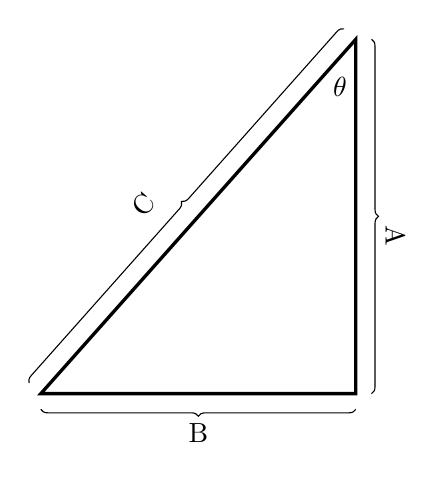
\begin{tikzpicture}
		    \coordinate (C) at (0,2);
		    \coordinate (D) at (4,2);
		    \coordinate (E) at (4,6.5);
		    %\tkzMarkRightAngle(C,D,E)
		    %\tkzMarkAngle(C,E,D)
		    \draw[decoration={brace,mirror,raise=.2cm},decorate,thin] (0,2)--(4,2);
		    \draw[decoration={brace,mirror,raise=.2cm},decorate,thin] (4,2)--(4,6.5);
		    \draw[decoration={brace,raise=.2cm},decorate,thin] (0,2)--(4,6.5);
		    \draw[very thick] (D)--(E)--(C)--cycle;
		    \node at (2,2-.5) {B};
		    \node[rotate=-90] at (4+.5,4) {A};
		    \node[rotate=48.5] at (1.4-.1,3.8+.6) {C};
		    \node at (3.8,5.9) {$\theta$};
		  \end{tikzpicture}
		\end{image}

Label all known lengths with units.
\begin{enumerate}
\item Side $A$ is the \wordChoice{\choice{base}\choice[correct]{mast}} and it is $\answer{8}$ m tall.

\item Side $B$ is the \wordChoice{\choice[correct]{base}\choice{mast}}.

\item Side $C$ is the diagonal of the sail and it is $\answer{\frac{16}{3}\sqrt{3}}$ $\answer{m}$ long.
\end{enumerate}

\item At what angle, $\theta$ (in radians), must you cut from the top of the sail to get the sail in the right shape? $\answer{\frac{\pi}{6}}$

\item How long will the base of the sail be (give units)? $\answer{\frac{8}{3}\sqrt{3}}$ $\answer{m}$

\item What is the surface area of the sail (give units)? $\answer{\frac{32}{3}\sqrt{3}}$ $\answer{m^2}$

\end{enumerate}

\end{exercise}
\end{document}
